% =====================================================================
%  Memoria - Actividad 2 (Grupal)
%  Razonamiento y Planificacion Automatica (MIA - RYPA)
%  Planificacion para un rover marciano
%
%  Formato exigido por la rubrica:
%    - Calibri o similar, 12 pt, interlineado 1.5
%    - Entrega exclusivamente en PDF
%    - Maximo 8 paginas SIN contar caratula ni apendices
%
%  Compilar con:  pdflatex muinar04_act2.tex   (dos veces)
%  Fuente: Carlito (clon libre metricamente compatible con Calibri).
%  Si no esta instalada:  tlmgr install carlito
%  Alternativa: comentar la linea de carlito y usar \usepackage{lmodern}
% =====================================================================

\documentclass[12pt,a4paper]{article}

% ---------- Codificacion e idioma ----------
\usepackage[T1]{fontenc}
\usepackage[utf8]{inputenc}
\usepackage[spanish,es-nodecimaldot,es-noshorthands]{babel}

% ---------- Tipografia: Calibri (via Carlito) ----------
\usepackage[sfdefault]{carlito}
\renewcommand{\familydefault}{\sfdefault}

% ---------- Geometria e interlineado ----------
\usepackage[a4paper,top=2.5cm,bottom=2.5cm,left=3cm,right=3cm]{geometry}
\usepackage{setspace}
\onehalfspacing

% ---------- Paquetes de contenido ----------
\usepackage{graphicx}
\usepackage{booktabs}
\usepackage{array}
\usepackage{longtable}
\usepackage{caption}
\usepackage{subcaption}
\usepackage{enumitem}
\usepackage{listings}
\usepackage{xcolor}
\usepackage{float}
\usepackage{fancyhdr}
\usepackage[hidelinks]{hyperref}

% Las imagenes van en la MISMA carpeta que este .tex, sin subcarpetas.
% La segunda ruta es solo un respaldo para compilar desde el repositorio.
\graphicspath{{./}{../../images/}}

% ---------- Encabezado y pie ----------
\pagestyle{fancy}
\fancyhf{}
\fancyhead[L]{\footnotesize Razonamiento y Planificaci\'on Autom\'atica}
\fancyhead[R]{\footnotesize Actividad 2 -- Rovers}
\fancyfoot[C]{\thepage}
\renewcommand{\headrulewidth}{0.4pt}

% ---------- Estilo para codigo PDDL ----------
\definecolor{pddlcomment}{RGB}{110,110,110}
\definecolor{pddlkey}{RGB}{0,90,160}
\definecolor{pddlbg}{RGB}{247,247,247}

\lstdefinelanguage{PDDL}{
  morekeywords={define,domain,problem,objects,init,goal,requirements,types,
                predicates,action,parameters,precondition,effect,and,not,or,when,forall},
  sensitive=false,
  morecomment=[l]{;},
}

\lstset{
  language=PDDL,
  basicstyle=\ttfamily\scriptsize,
  keywordstyle=\color{pddlkey}\bfseries,
  commentstyle=\color{pddlcomment}\itshape,
  backgroundcolor=\color{pddlbg},
  frame=single,
  rulecolor=\color{gray!40},
  breaklines=true,
  columns=fullflexible,
  showstringspaces=false,
  xleftmargin=0.5em,
  framexleftmargin=0.5em,
  aboveskip=0.6em,
  belowskip=0.6em,
}

% ---------- Espaciado de listas mas compacto ----------
\setlist[itemize]{topsep=2pt,itemsep=1pt,parsep=0pt}
\setlist[enumerate]{topsep=2pt,itemsep=1pt,parsep=0pt}

% ---------- Titulos de seccion ----------
\usepackage{titlesec}
\titlespacing*{\section}{0pt}{1.2ex plus 1ex minus .2ex}{0.8ex plus .2ex}
\titlespacing*{\subsection}{0pt}{1.0ex plus 1ex minus .2ex}{0.6ex plus .2ex}

% ---------- Bibliografia APA manual (sangria francesa) ----------
\newenvironment{referencias}
  {\begin{list}{}{%
      \setlength{\leftmargin}{1.25cm}%
      \setlength{\itemindent}{-1.25cm}%
      \setlength{\itemsep}{0.6em}%
      \setlength{\parsep}{0pt}}}
  {\end{list}}

% =====================================================================
\begin{document}

% ---------------------------------------------------------------------
% CARATULA (no cuenta para el limite de 8 paginas)
% ---------------------------------------------------------------------
\begin{titlepage}
\centering
\vspace*{2cm}

{\Large\bfseries M\'aster Universitario en Inteligencia Artificial\par}
\vspace{0.4cm}
{\large Razonamiento y Planificaci\'on Autom\'atica\par}

\vspace{2.5cm}
{\Huge\bfseries Actividad 2 (Grupal)\par}
\vspace{0.6cm}
{\LARGE Planificaci\'on para un rover marciano\par}
\vspace{0.4cm}
{\large Especificaci\'on, resoluci\'on y evaluaci\'on de un dominio PDDL\par}

\vspace{3cm}
{\large\bfseries Autores\par}
\vspace{0.3cm}
{\large
% TODO: sustituir por los nombres completos de los integrantes del grupo
Isaac Cerda\\[2pt]
[Nombre del segundo integrante]\\[2pt]
[Nombre del tercer integrante]\\[2pt]
[Nombre del cuarto integrante]\par}

\vfill
{\large Curso 2025--2026\par}
\vspace{0.3cm}
{\large \today\par}
\end{titlepage}

% ---------------------------------------------------------------------
% El contador se reinicia: la caratula no cuenta
% ---------------------------------------------------------------------
\setcounter{page}{1}

% =====================================================================
\section{Parte 1. Entorno de desarrollo y conceptos b\'asicos}
% =====================================================================

\subsection{1.1. Instalaci\'on y prueba del entorno}

Se ha utilizado \textbf{Visual Studio Code} con la extensi\'on \textbf{PDDL}
de Jan Dolejsi (\texttt{jan-dolejsi.pddl}, versi\'on 2.28.2), configurada
contra el servicio remoto \emph{Planning as a Service}
(\url{https://solver.planning.domains:5001/package}), seleccionando el motor
\texttt{dual-bfws-ffparser}. Los ficheros \texttt{.pddl} se editan y validan
en local y la resoluci\'on se delega en el servicio remoto, de modo que no
ha sido necesario compilar ning\'un planificador en la m\'aquina propia.

Ejecutando el dominio y el problema base proporcionados con la actividad, el
entorno resuelve el caso correctamente: el \emph{parser} instancia
82 acciones sobre 40 \emph{fluents} y se encuentra un
\textbf{plan de coste 12}, tras \textbf{generar 166 nodos y expandir 113}
mediante la b\'usqueda \emph{Fast-BFS} (1-BFWS). El plan satisface los tres
objetivos del problema: comunicar la imagen de alta resoluci\'on del
\texttt{objective1}, la muestra de suelo de \texttt{waypoint2} y la muestra
de roca de \texttt{waypoint3}. Las capturas que evidencian la instalaci\'on
y la ejecuci\'on se recogen en el Ap\'endice
(figuras~\ref{fig:vscode}--\ref{fig:planbase}).

\subsection{1.2. Encadenamiento hacia delante: acciones aplicables en el
primer paso}

Un planificador de encadenamiento hacia delante parte del estado inicial y
selecciona las acciones instanciadas cuyas precondiciones son todas ciertas
en \'el. El razonamiento seguido ha sido recorrer cada operador del dominio
y filtrar sus par\'ametros precondici\'on a precondici\'on, descartando en
cuanto una de ellas no se satisface.

\paragraph{\texttt{navigate-bat}.}
Sus precondiciones son \texttt{can\_traverse}, \texttt{available},
\texttt{at}, \texttt{visible}, \texttt{battery\_installed} y \texttt{lower}.
En el estado inicial existen seis hechos \texttt{can\_traverse} para
\texttt{rover0}, pero \texttt{(at rover0 waypoint1)} obliga a que el
movimiento parta de \texttt{waypoint1}, lo que deja s\'olo los destinos
\texttt{waypoint2} y \texttt{waypoint3}. Ambos son adem\'as visibles desde
\texttt{waypoint1} (\texttt{(visible waypoint1 waypoint2)} y
\texttt{(visible waypoint1 waypoint3)}), por lo que ninguno se descarta.
Existe un \'unico hecho de bater\'ia,
\texttt{(battery\_installed rover0 bat0 b4 b2)}, que fija
\texttt{?b\,=\,bat0}, \texttt{?bmax\,=\,b4} y \texttt{?bcur\,=\,b2};
la precondici\'on \texttt{(lower ?bnext ?bcur)} con \texttt{?bcur\,=\,b2}
s\'olo admite \texttt{(lower b1 b2)}, luego \texttt{?bnext\,=\,b1}. Quedan
dos instancias aplicables.

\paragraph{\texttt{recharge}.}
Exige que rover y \emph{lander} coincidan de posici\'on. El rover est\'a en
\texttt{waypoint1} y \texttt{(at\_lander general waypoint2)}, por lo que
\textbf{no es aplicable}.

\paragraph{\texttt{sample\_soil}.}
Requiere \texttt{(at\_soil\_sample ?p)} con \texttt{?p\,=\,waypoint1}, pero
las muestras de suelo est\'an en \texttt{waypoint0}, \texttt{waypoint2} y
\texttt{waypoint3}. \textbf{No aplicable}.

\paragraph{\texttt{sample\_rock}.}
S\'i existe \texttt{(at\_rock\_sample waypoint1)}. Adem\'as se cumplen
\texttt{(equipped\_for\_rock\_analysis rover0)},
\texttt{(store\_of rover0store rover0)} y \texttt{(empty rover0store)}.
\textbf{Aplicable}.

\paragraph{\texttt{drop}.}
Pide \texttt{(full ?s)}, pero el almac\'en est\'a vac\'io.
\textbf{No aplicable}.

\paragraph{\texttt{calibrate}.}
Se cumplen \texttt{(equipped\_for\_imaging rover0)},
\texttt{(calibration\_target camera0 objective1)} --- \'unico hecho de este
tipo, lo que fija c\'amara y objetivo ---,
\texttt{(visible\_from objective1 waypoint1)} y
\texttt{(on\_board camera0 rover0)}. \textbf{Aplicable}. N\'otese que
\texttt{objective0} no aparece como \texttt{calibration\_target} y por eso
no genera alternativas.

\paragraph{\texttt{take\_image}.}
Exige \texttt{(calibrated ?i ?r)}, que no est\'a en el estado inicial porque
s\'olo se produce como efecto de \texttt{calibrate}. \textbf{No aplicable}.

\paragraph{Acciones \texttt{communicate\_*}.}
Las tres fallan por el mismo motivo: requieren
\texttt{have\_soil\_analysis}, \texttt{have\_rock\_analysis} o
\texttt{have\_image}, que son efectos de las acciones de muestreo y de
captura de imagen y a\'un no se han producido. \textbf{No aplicables}.

\medskip
En consecuencia, un planificador de encadenamiento hacia delante dispone en
el primer paso de \textbf{cuatro acciones instanciadas}:

\begin{lstlisting}
(navigate-bat rover0 waypoint1 waypoint2 bat0 b4 b2 b1)
(navigate-bat rover0 waypoint1 waypoint3 bat0 b4 b2 b1)
(sample_rock  rover0 rover0store waypoint1)
(calibrate    rover0 camera0 objective1 waypoint1)
\end{lstlisting}

\subsection{1.3. Encadenamiento hacia atr\'as: acciones consideradas desde
el objetivo}

Un planificador de encadenamiento hacia atr\'as parte del \emph{goal} y
busca, para cada literal objetivo, las acciones que lo producen en sus
efectos, unificando los par\'ametros. Una precondici\'on no satisfecha en el
estado inicial no descarta la acci\'on: simplemente pasa a ser un
subobjetivo pendiente. El razonamiento clave que hemos aplicado en los tres
casos es que \texttt{visible} y \texttt{at\_lander} \textbf{no aparecen en
el efecto de ning\'un operador} del dominio base, por lo que son
literales est\'aticos y sus valores s\'olo pueden tomarse del estado
inicial: eso permite fijar \texttt{?y\,=\,waypoint2} y acotar \texttt{?x} a
tres posibilidades.

\paragraph{Objetivo \texttt{(communicated\_soil\_data waypoint2)}.}
Lo produce \texttt{communicate\_soil\_data}, que unifica
\texttt{?p\,=\,waypoint2}. Al existir un solo rover y un solo \emph{lander},
\texttt{?r\,=\,rover0} y \texttt{?l\,=\,general}. De
\texttt{(at\_lander general waypoint2)} se deduce \texttt{?y\,=\,waypoint2},
y de \texttt{(visible ?x waypoint2)} se obtienen tres valores posibles para
\texttt{?x}: \texttt{waypoint0}, \texttt{waypoint1} y \texttt{waypoint3}
(obs\'ervese que \texttt{waypoint2} no es visible desde s\'i mismo). La
precondici\'on \texttt{(have\_soil\_analysis rover0 waypoint2)} queda como
subobjetivo.

\paragraph{Objetivo \texttt{(communicated\_rock\_data waypoint3)}.}
An\'alogamente con \texttt{communicate\_rock\_data}, unificando
\texttt{?p\,=\,waypoint3} y quedando
\texttt{(have\_rock\_analysis rover0 waypoint3)} como subobjetivo.

\paragraph{Objetivo \texttt{(communicated\_image\_data objective1 high\_res)}.}
Con \texttt{communicate\_image\_data}, unificando \texttt{?o\,=\,objective1}
y \texttt{?m\,=\,high\_res}, y dejando
\texttt{(have\_image rover0 objective1 high\_res)} como subobjetivo, que a su
vez exigir\'a \texttt{calibrate} y \texttt{take\_image}.

\medskip
Se consideran por tanto \textbf{nueve acciones instanciadas} en el primer
paso, tres por cada literal del objetivo:

\begin{lstlisting}
(communicate_soil_data  rover0 general waypoint2 {waypoint0|waypoint1|waypoint3} waypoint2)
(communicate_rock_data  rover0 general waypoint3 {waypoint0|waypoint1|waypoint3} waypoint2)
(communicate_image_data rover0 general objective1 high_res {waypoint0|waypoint1|waypoint3} waypoint2)
\end{lstlisting}

\subsection{1.4. Ejecuci\'on del caso base y an\'alisis de la traza}

\paragraph{Planificador y configuraci\'on.}
Se ha empleado \textbf{BFWS \emph{dual} con \emph{parser} de FF}
(\texttt{dual-bfws-ffparser}), ejecutado como servicio remoto sin opciones
adicionales. Es un planificador \emph{satisfactorio} (SAT): garantiza
encontrar una soluci\'on v\'alida si existe, pero no que sea \'optima. Se ha
elegido por ser uno de los planificadores de referencia de la actividad y
por ser plenamente compatible con PDDL 1.2.

\paragraph{Interpretaci\'on de la traza.}
Seg\'un Lipovetzky y Geffner (2017), BFWS ordena la frontera de b\'usqueda
combinando la \emph{novedad} de los estados con dos medidas de progreso
hacia la meta. En la traza esto se observa en los pares del tipo
\texttt{[3/2]}: el primer valor, $\#g$, es el n\'umero de objetivos que
todav\'ia no se han alcanzado, y el segundo, $\#r$, cuenta los hechos
\'utiles del \'ultimo plan relajado ya conseguidos. Por eso $\#g$ desciende
progresivamente de 3 a 0 conforme se van satisfaciendo los tres literales
del \emph{goal}.

La configuraci\'on \emph{dual} encadena dos b\'usquedas: primero
\textbf{1-BFWS}, que restringe la exploraci\'on a estados de novedad 1 y es
muy r\'apida, y s\'olo si \'esta fracasa se lanza una segunda b\'usqueda m\'as
completa. \textbf{En nuestro caso no fue necesaria la segunda pasada}, porque
1-BFWS encontr\'o directamente un plan v\'alido.

\paragraph{Resultado y m\'etricas.}
Se obtuvo un plan de \textbf{12 acciones y coste 12} (todas las acciones del
dominio tienen coste unitario), generando \textbf{166 nodos} y expandiendo
\textbf{113}, en un tiempo de b\'usqueda del orden de $5\cdot10^{-4}$~s. La
relaci\'on generados/expandidos ($\approx 1{,}47$) indica una b\'usqueda muy
dirigida, con poco ramificado descartado, coherente con un problema peque\~no
y una heur\'istica informativa.

\paragraph{Comentario del plan.}
El plan es sensato y sin desperdicio: el rover aprovecha que \texttt{objective1}
es visible desde su posici\'on inicial para calibrar, fotografiar y comunicar
la imagen sin moverse; despu\'es viaja a \texttt{waypoint2}, recarga
aprovechando que all\'i est\'a el \emph{lander}, toma la muestra de suelo y
regresa a \texttt{waypoint1} para comunicarla --- movimiento obligado, ya
que \texttt{waypoint2} no es visible desde s\'i mismo ---; finalmente se
desplaza a \texttt{waypoint3}, vac\'ia el almac\'en, toma la muestra de roca
y la comunica.

\paragraph{Nota sobre las marcas temporales.}
El valor \texttt{0.011} que aparece junto a la \'ultima acci\'on de la traza
es la \emph{marca temporal} de esa acci\'on en el plan (las acciones se
espacian $0{,}001$), no el coste del plan. El coste sigue siendo 12.

% =====================================================================
\section{Parte 2. Modificaci\'on del estado inicial y objetivos}
% =====================================================================

En esta parte se modifica \'unicamente el fichero de problema; el dominio se
mantiene byte a byte id\'entico al original. Los dos casos se han resuelto de
forma independiente, partiendo cada uno del problema inicial.

\subsection{2.1. Nuevo \emph{waypoint} con muestras y retorno a
\texttt{waypoint1}}

\paragraph{Dise\~no de la soluci\'on.}
Se a\~nade el objeto \texttt{waypoint4} y las muestras que debe contener:

\begin{lstlisting}
(at_soil_sample waypoint4)
(at_rock_sample waypoint4)
\end{lstlisting}

La decisi\'on sobre \emph{con qu\'e dos waypoints} conectarlo no es
arbitraria, sino que se deriva de las precondiciones de
\texttt{communicate\_soil\_data} y \texttt{communicate\_rock\_data}. \'Estas
exigen \texttt{(at\_lander ?l ?y)} y \texttt{(visible ?x ?y)}: como el
\emph{lander} est\'a en \texttt{waypoint2}, para poder comunicar desde el
propio \texttt{waypoint4} hace falta \texttt{(visible waypoint4 waypoint2)}.
Conectarlo adem\'as con \texttt{waypoint2} permite al planificador recargar
si lo necesita, ya que es la posici\'on del \emph{lander}. El segundo enlace
se hace con \texttt{waypoint1}, que es donde el rover parte y donde debe
terminar. Ambas conexiones se declaran en las dos direcciones, tanto en
visibilidad como en transitabilidad:

\begin{lstlisting}
; Visibilidad de waypoint4 con waypoint1 y waypoint2, bidireccional
(visible waypoint1 waypoint4) (visible waypoint4 waypoint1)
(visible waypoint2 waypoint4) (visible waypoint4 waypoint2)
; Transitabilidad del rover hacia y desde waypoint4
(can_traverse rover0 waypoint1 waypoint4) (can_traverse rover0 waypoint4 waypoint1)
(can_traverse rover0 waypoint2 waypoint4) (can_traverse rover0 waypoint4 waypoint2)
\end{lstlisting}

Finalmente se a\~naden los tres objetivos pedidos:

\begin{lstlisting}
(communicated_soil_data waypoint4)
(communicated_rock_data waypoint4)
(at rover0 waypoint1)          ; el rover debe terminar en waypoint1
\end{lstlisting}

\paragraph{Resultado.}
El planificador encuentra un \textbf{plan de coste 20}, generando
\textbf{369 nodos} y expandiendo \textbf{181}. El an\'alisis detallado se
desarrolla en la secci\'on~3.1.

\subsection{2.2. Segundo rover con capacidad de movimiento y fotograf\'ia}

\paragraph{Dise\~no de la soluci\'on.}
Se a\~naden los objetos \texttt{rover1}, \texttt{bat1} y \texttt{camera1},
\textbf{sin tocar ning\'un hecho relativo a \texttt{rover0}}. El nuevo rover
se declara \texttt{(available rover1)} y se sit\'ua en
\texttt{(at rover1 waypoint0)}: se ha elegido \texttt{waypoint0} porque desde
ah\'i son visibles \emph{todos} los objetivos, lo que le permite empezar a
trabajar de inmediato. Situarlo en \texttt{waypoint3}, por ejemplo, habr\'ia
sido peor, porque desde all\'i no alcanza \texttt{objective1}.

Como s\'olo debe tener capacidad de movimiento y fotograf\'ia,
\textbf{no se le asigna almac\'en} ni predicados
\texttt{equipped\_for\_*\_analysis}; s\'i
\texttt{(equipped\_for\_imaging rover1)}. La c\'amara se monta con
\texttt{(on\_board camera1 rover1)}, se declara calibrable contra ambos
objetivos y compatible con los tres modos:

\begin{lstlisting}
(calibration_target camera1 objective0) (calibration_target camera1 objective1)
(supports camera1 colour) (supports camera1 low_res) (supports camera1 high_res)
\end{lstlisting}

\paragraph{Justificaci\'on del nivel m\'aximo de bater\'ia.}
La bater\'ia se instala con \texttt{(battery\_installed rover1 bat1 b4 b2)},
es decir, nivel inicial \texttt{b2} como pide el enunciado y \emph{m\'aximo}
\texttt{b4} en lugar de \texttt{b5}. La raz\'on es que la precondici\'on
\texttt{(lower ?bnext ?bcur)} de \texttt{navigate-bat} exige que exista un
nivel estrictamente inferior al actual, y en el problema no hay ning\'un
hecho \texttt{lower} cuyo segundo argumento sea \texttt{b5}: si el m\'aximo
fuera \texttt{b5}, el rover quedar\'ia \textbf{bloqueado justo despu\'es de
recargar}, sin poder moverse. Este detalle es una consecuencia sutil de
modelar la bater\'ia con niveles discretos en lugar de \emph{fluents}
num\'ericos.

\paragraph{Rutas y objetivos.}
Se replican para \texttt{rover1} las rutas de \texttt{rover0} y se a\~naden
enlaces adicionales con \texttt{waypoint2} para que pueda acudir al
\emph{lander} a recargar si lo necesita. Los objetivos se ampl\'ian hasta
cubrir \emph{todas} las muestras del problema y \emph{todas} las
combinaciones objetivo--modo:

\begin{lstlisting}
(communicated_soil_data waypoint0) (communicated_soil_data waypoint3)
(communicated_rock_data waypoint1) (communicated_rock_data waypoint2)
(communicated_image_data objective0 colour)  (communicated_image_data objective0 high_res)
(communicated_image_data objective0 low_res) (communicated_image_data objective1 colour)
(communicated_image_data objective1 low_res)
\end{lstlisting}

Junto con los tres objetivos originales suman \textbf{12 metas}: 6 de
muestras (suelo en \texttt{waypoint0}, \texttt{waypoint2} y
\texttt{waypoint3}; roca en \texttt{waypoint1}, \texttt{waypoint2} y
\texttt{waypoint3}) y 6 de imagen (dos objetivos $\times$ tres modos).

\paragraph{Resultado.}
El planificador resuelve el caso con un \textbf{plan de coste 45},
generando \textbf{736 nodos} y expandiendo \textbf{392}, lo que confirma que
el modelo es consistente y que no falta ning\'un elemento para satisfacer el
enunciado. El an\'alisis se desarrolla en la secci\'on~3.2.

% =====================================================================
\section{Parte 3. Ejecuci\'on y evaluaci\'on del planificador}
% =====================================================================

Todas las ejecuciones se han realizado con \texttt{dual-bfws-ffparser} a
trav\'es de \texttt{solver.planning.domains:5001}, sin opciones adicionales,
resolviendo en todos los casos con la primera b\'usqueda (\textbf{1-BFWS}).
La tabla~\ref{tab:metricas} resume las m\'etricas comparadas.

\begin{table}[H]
\centering
\caption{M\'etricas comparadas de las tres ejecuciones
(\texttt{dual-bfws-ffparser}, b\'usqueda 1-BFWS).}
\label{tab:metricas}
\small
\begin{tabular}{lrrr}
\toprule
\textbf{M\'etrica} & \textbf{Caso inicial} & \textbf{Caso 2.1} & \textbf{Caso 2.2} \\
\midrule
Coste del plan (acciones)      & 12       & 20       & 45       \\
Nodos generados                & 166      & 369      & 736      \\
Nodos expandidos               & 113      & 181      & 392      \\
Metas detectadas               & 3        & 6        & 12       \\
Acciones instanciadas          & 82       & 118      & 172      \\
Predicados del estado          & 40       & 47       & 59       \\
Tiempo de b\'usqueda (s)        & 0,000502 & 0,001586 & 0,002989 \\
\emph{Makespan} (simulado)     & 0,011    & 0,019    & 0,044    \\
Planes encontrados             & 1        & 1        & 1        \\
\bottomrule
\end{tabular}

\vspace{0.4em}
{\footnotesize\emph{Nota}: los tiempos corresponden a una ejecuci\'on de
referencia; al tratarse de un servicio remoto var\'ian ligeramente entre
ejecuciones (del orden del 10\,\%), mientras que coste, nodos y metas son
deterministas y reproducibles.}
\end{table}

\subsection{3.1. An\'alisis del caso 2.1 y comparaci\'on con el caso inicial}

\paragraph{Comentario general del plan.}
El rover empieza aprovechando su posici\'on: calibra la c\'amara, fotograf\'ia
\texttt{objective1} y comunica la imagen sin moverse de \texttt{waypoint1}.
A continuaci\'on viaja a \texttt{waypoint4}, donde toma y comunica la muestra
de suelo, vac\'ia el almac\'en y repite con la de roca --- puede comunicar
desde all\'i mismo gracias a la visibilidad que a\~nadimos con
\texttt{waypoint2}. Despu\'es se desplaza a \texttt{waypoint2}, vac\'ia,
toma la muestra de suelo, recarga y viaja a \texttt{waypoint1} para
comunicarla. Finalmente va a \texttt{waypoint3}, toma la muestra de roca, la
comunica y regresa a \texttt{waypoint1} para cumplir el objetivo de posici\'on
final.

\paragraph{\textquestiondown Hay movimientos innecesarios?}
\textbf{S\'i}. El caso m\'as claro se produce cuando el rover est\'a en
\texttt{waypoint2} con la muestra de suelo de ese punto: para comunicarla
necesita visibilidad hacia \texttt{waypoint2}, que se obtiene desde
\texttt{waypoint1} \emph{o} desde \texttt{waypoint3}. El planificador elige
ir a \texttt{waypoint1}, comunicar, y \emph{despu\'es} viajar vac\'io hasta
\texttt{waypoint3}. Una alternativa equivalente en objetivos habr\'ia sido ir
directamente a \texttt{waypoint3}, comunicar desde all\'i, tomar la muestra
de roca y cerrar el recorrido en \texttt{waypoint1}, ahorrando un
desplazamiento.

\paragraph{\textquestiondown Por qu\'e ocurre?}
Por la naturaleza \textbf{satisfactoria y no \'optima} del planificador. BFWS
prioriza estados por novedad y por cercan\'ia heur\'istica al objetivo, no por
coste acumulado real; en cuanto encuentra un plan v\'alido termina, sin
explorar si exist\'ia otro m\'as corto. Adem\'as, la heur\'istica de plan
relajado ignora los efectos negativos, de modo que \texttt{waypoint1} y
\texttt{waypoint3} le resultan pr\'acticamente indistinguibles como puntos de
comunicaci\'on y desempata por el orden interno de generaci\'on de sucesores.
A esto se suma que el objetivo \texttt{(at rover0 waypoint1)} sesga la
heur\'istica a favor de visitar \texttt{waypoint1}, aunque en ese instante
del plan la visita sea prematura.

\paragraph{Comparaci\'on con el caso inicial.}
El coste pasa de 12 a 20 ($+67\,\%$), consecuencia directa de a\~nadir tres
objetivos (dos comunicaciones en \texttt{waypoint4} y la posici\'on final) y
un \emph{waypoint} m\'as. El esfuerzo de b\'usqueda crece en proporci\'on
similar: 369 frente a 166 nodos generados ($\times2{,}2$) y 181 frente a 113
expandidos ($\times1{,}6$). Es interesante que los nodos expandidos crezcan
\emph{menos} que los generados: la restricci\'on adicional de terminar en
\texttt{waypoint1} poda parte del espacio y mantiene la b\'usqueda dirigida.
El tiempo se triplica pero permanece en el orden del milisegundo, es decir,
el aumento de complejidad es perfectamente asumible a esta escala.

\subsection{3.2. An\'alisis del caso 2.2 y comparaci\'on con el plan original}

\paragraph{Comentario general del plan.}
\texttt{rover0} arranca en \texttt{waypoint1} tomando y comunicando la muestra
de roca, y fotograf\'ia \texttt{objective1} en \texttt{high\_res} y
\texttt{objective0} en \texttt{colour}. \texttt{rover1} entra en acci\'on desde
\texttt{waypoint0} y cubre las cuatro im\'agenes restantes
(\texttt{objective1/colour}, \texttt{objective0/high\_res},
\texttt{objective0/low\_res}, \texttt{objective1/low\_res}) sin moverse en
ning\'un momento. A partir de ah\'i, \texttt{rover0} asume en solitario toda
la recolecci\'on de muestras, encadenando viajes entre \texttt{waypoint1},
\texttt{waypoint2}, \texttt{waypoint3} y \texttt{waypoint0}, con dos recargas
intermedias en el \emph{lander}.

\paragraph{\textquestiondown Utiliza el plan a \texttt{rover1}?}
\textbf{S\'i}, y lo hace de forma coherente con sus capacidades: se encarga de
6 de las acciones del plan, todas fotogr\'aficas, exactamente aquello para lo
que fue definido en el problema.

\paragraph{\textquestiondown Lo hace de la mejor forma posible?}
\textbf{No, y la limitaci\'on es de modelado, no del planificador.} Al haberse
especificado \texttt{rover1} \'unicamente como ``fot\'ografo'' --- sin
almac\'en ni equipamiento de an\'alisis, tal como exige el enunciado --- todo
el trabajo de muestreo recae obligatoriamente sobre \texttt{rover0}, que es
adem\'as el \'unico con almac\'en. El paralelismo real es por tanto muy
limitado: \texttt{rover1} ni siquiera necesita desplazarse, porque desde
\texttt{waypoint0} ve ambos objetivos. Si se le hubieran otorgado capacidades
de an\'alisis, el trabajo se habr\'ia repartido y el plan ser\'ia
sensiblemente m\'as corto.

\paragraph{\textquestiondown Por qu\'e se da este efecto?}
Adem\'as de la restricci\'on de capacidades, influye un factor estructural del
dominio: el predicado \texttt{channel\_free} y la secuencia
\texttt{(not (available ?r))\dots(available ?r)} dentro de las acciones
\texttt{communicate\_*} \textbf{serializan} las comunicaciones. Como el plan
es una secuencia totalmente ordenada de acciones de coste unitario, a\~nadir
un segundo agente \emph{no reduce el coste}: reparte el trabajo, pero la
m\'etrica sigue contando acciones, no tiempo transcurrido. Un planificador
temporal con acciones dur\'ativas s\'i habr\'ia reflejado el beneficio del
paralelismo.

\paragraph{Comparaci\'on con el plan original.}
El coste se multiplica por 3,75 (45 frente a 12), pero el n\'umero de metas se
cuadruplica (12 frente a 3): el crecimiento es aproximadamente proporcional a
la carga de trabajo, no explosivo. Los nodos generados pasan de 166 a 736
($\times4{,}4$) y los expandidos de 113 a 392 ($\times3{,}5$), y el tiempo de
b\'usqueda se multiplica por seis, aunque sigue por debajo de los 3~ms. El
espacio de estados crece adem\'as por la ramificaci\'on adicional que introduce
un segundo agente: 172 acciones instanciadas frente a 82.

\subsection{3.3. Conclusiones}

\begin{enumerate}[leftmargin=*]
\item \textbf{El coste crece con el n\'umero de metas, no con el n\'umero de
agentes.} A\~nadir \texttt{rover1} no abarat\'o el plan; lo que lo encareci\'o
fue pasar de 3 a 12 objetivos. En un dominio STRIPS de coste unitario y plan
totalmente ordenado, el paralelismo no se recompensa.

\item \textbf{La b\'usqueda se mantiene muy dirigida en los tres casos.} La
raz\'on generados/expandidos oscila entre 1,47 y 2,04, se\~nal de que la
combinaci\'on de novedad y heur\'istica de plan relajado descarta poco
material \'util. Sin embargo, esa raz\'on crece con la complejidad, lo que
anticipa una degradaci\'on en instancias mayores.

\item \textbf{Ser satisfactorio tiene un precio observable.} Los movimientos
redundantes detectados en 3.1 son el s\'intoma directo de que BFWS detiene la
b\'usqueda en el primer plan v\'alido. Un planificador \'optimo (por ejemplo,
A$^\ast$ con una heur\'istica admisible) habr\'ia eliminado ese
desplazamiento, a costa de un esfuerzo de b\'usqueda muy superior. En
problemas reales de exploraci\'on planetaria, donde la energ\'ia es el recurso
cr\'itico, ese compromiso debe evaluarse expl\'icitamente.

\item \textbf{Las decisiones de modelado condicionan el plan tanto como el
algoritmo.} La elecci\'on de \texttt{b4} como m\'aximo de bater\'ia, la
posici\'on inicial de \texttt{rover1} o la ausencia de
\texttt{(visible waypoint2 waypoint2)} determinan planes completamente
distintos. Buena parte del ``comportamiento extra\~no'' de un planificador se
explica revisando el problema, no el algoritmo.
\end{enumerate}

% =====================================================================
\section{Parte 4. Modificaci\'on del dominio}
% =====================================================================

\subsection{4.1. Descripci\'on de la soluci\'on}

Se han introducido tres cambios sobre el dominio base, todos ellos
\textbf{gen\'ericos}, es decir, independientes del n\'umero y del nombre de
los rovers y \emph{landers} presentes en el problema concreto.

\paragraph{(1) Nuevo predicado \texttt{suitable\_for\_lander}.}

\begin{lstlisting}
; NUEVO (Parte 4): waypoint fisicamente apto para el lander
(suitable_for_lander ?w - waypoint)
\end{lstlisting}

Marca qu\'e \emph{waypoints} son f\'isicamente adecuados para que el
\emph{lander} sea utilizable ah\'i: suficiente radiaci\'on solar para servir
de punto de repostaje y posibilidad de comunicaci\'on con la Tierra. Es
deliberadamente \textbf{unario sobre \texttt{waypoint}} y no binario sobre
$(lander, waypoint)$: la aptitud es una propiedad del terreno, no del
veh\'iculo, de modo que la representaci\'on sigue siendo v\'alida con
cualquier n\'umero de \emph{landers} sin duplicar hechos.

\paragraph{(2) Restricci\'on de los operadores que usan el \emph{lander}.}
Las cuatro acciones en las que participa el \emph{lander} ---
\texttt{recharge}, \texttt{communicate\_soil\_data},
\texttt{communicate\_rock\_data} y \texttt{communicate\_image\_data} ---
incorporan la nueva precondici\'on sobre el \emph{waypoint} donde \'este se
encuentra:

\begin{lstlisting}
(:action communicate_soil_data
 :parameters (?r - rover ?l - lander ?p - waypoint ?x - waypoint ?y - waypoint)
 :precondition (and (at ?r ?x) (at_lander ?l ?y) (have_soil_analysis ?r ?p)
                    (visible ?x ?y) (available ?r) (channel_free ?l)
                    ; NUEVO (Parte 4): el lander debe estar en un waypoint apto
                    (suitable_for_lander ?y))
 ...)
\end{lstlisting}

Si el \emph{lander} no est\'a en un emplazamiento adecuado, ninguna de estas
acciones es aplicable: queda efectivamente inutilizado, que es justo lo que
pide el enunciado.

\paragraph{(3) Nuevo operador \texttt{tow\_lander}.}

\begin{lstlisting}
(:action tow_lander
:parameters (?r1 ?r2 - rover ?l - lander ?y - waypoint ?z - waypoint
             ?b1 - battery ?bmax1 ?bcur1 ?bnext1 - blevel
             ?b2 - battery ?bmax2 ?bcur2 ?bnext2 - blevel)
:precondition (and (not (= ?r1 ?r2))
               (at ?r1 ?y) (at ?r2 ?y) (at_lander ?l ?y)
               (available ?r1) (available ?r2)
               (can_traverse ?r1 ?y ?z) (can_traverse ?r2 ?y ?z)
               (visible ?y ?z)
               (battery_installed ?r1 ?b1 ?bmax1 ?bcur1) (lower ?bnext1 ?bcur1)
               (battery_installed ?r2 ?b2 ?bmax2 ?bcur2) (lower ?bnext2 ?bcur2))
:effect (and (not (at ?r1 ?y)) (at ?r1 ?z)
             (not (at ?r2 ?y)) (at ?r2 ?z)
             (not (at_lander ?l ?y)) (at_lander ?l ?z)
             (not (battery_installed ?r1 ?b1 ?bmax1 ?bcur1))
             (battery_installed ?r1 ?b1 ?bmax1 ?bnext1)
             (not (battery_installed ?r2 ?b2 ?bmax2 ?bcur2))
             (battery_installed ?r2 ?b2 ?bmax2 ?bnext2)))
\end{lstlisting}

Su funcionamiento replica el de \texttt{navigate-bat} pero exigido
\emph{simult\'aneamente} a dos rovers:

\begin{itemize}[leftmargin=*]
\item \textbf{Rovers distintos}: \texttt{(not (= ?r1 ?r2))}, para lo que se
a\~nade el requisito \texttt{:equality} al dominio. Sin esta condici\'on, un
\'unico rover podr\'ia unificarse consigo mismo y remolcar el \emph{lander}
en solitario.
\item \textbf{Los tres veh\'iculos parten del mismo punto}: las tres
precondiciones \texttt{(at ?r1 ?y)}, \texttt{(at ?r2 ?y)} y
\texttt{(at\_lander ?l ?y)} comparten la variable \texttt{?y}, y los tres
efectos posicionales comparten \texttt{?z}. As\'i se garantiza que empiezan y
terminan juntos.
\item \textbf{Restricciones an\'alogas al movimiento normal}: se exige
\texttt{can\_traverse} para \emph{ambos} rovers y \texttt{visible} entre
origen y destino.
\item \textbf{Consumo de bater\'ia de los dos}: cada rover tiene su propio
juego de par\'ametros de bater\'ia y su propia condici\'on
\texttt{(lower ?bnextN ?bcurN)}, de modo que cada uno desciende un nivel. Se
mantiene el esquema de \textbf{niveles discretos} (\texttt{blevel} +
\texttt{lower}) ya presente en el dominio, sin recurrir a \emph{fluents}
num\'ericos ni a comparaciones, tal como exige PDDL 1.2.
\end{itemize}

\subsection{4.2. Fichero de dominio}

El nuevo dominio se entrega como \texttt{rovers\_parte4\_dominio.pddl}. Todas
las modificaciones est\'an marcadas con comentarios que empiezan por
\texttt{; NUEVO (Parte 4):}, adem\'as de una cabecera que resume los tres
cambios, de forma que sean inmediatamente localizables. Se ha evitado
cualquier car\'acter internacional, incluidos los comentarios.

\subsection{4.3. Caso de prueba}

El problema \texttt{rovers\_parte4\_problema.pddl} est\'a dise\~nado para que
la nueva funcionalidad sea \emph{imprescindible}, no meramente opcional:

\begin{itemize}[leftmargin=*]
\item El \emph{lander} \texttt{general} comienza en \texttt{waypoint0}, que
\textbf{no} es apto.
\item El \'unico \emph{waypoint} apto es \texttt{waypoint2}
(\texttt{(suitable\_for\_lander waypoint2)}).
\item \texttt{rover0} y \texttt{rover1} comienzan junto al \emph{lander} en
\texttt{waypoint0}, ambos con bater\'ia a nivel \texttt{b2} y m\'aximo
\texttt{b4}.
\item Los objetivos exigen comunicar suelo (\texttt{waypoint1}), roca
(\texttt{waypoint3}) e imagen (\texttt{objective1/high\_res}).
\end{itemize}

Puesto que todas las acciones \texttt{communicate\_*} y \texttt{recharge}
requieren ahora un \emph{lander} en emplazamiento apto, \textbf{ning\'un
objetivo es alcanzable} hasta que los dos rovers remolquen el \emph{lander}
hasta \texttt{waypoint2}. Tras el remolque, cada rover se especializa
(\texttt{rover0} $\rightarrow$ suelo en \texttt{waypoint1} y fotograf\'ia;
\texttt{rover1} $\rightarrow$ roca en \texttt{waypoint3}) y ambos pueden
comunicar desde donde terminan, ya que el grafo de visibilidad entre los
cuatro \emph{waypoints} es completo.

\subsection{4.4. Ejecuci\'on y an\'alisis}

\paragraph{Resultados con los dos planificadores de referencia.}
El caso se ha resuelto con ambos planificadores de referencia; los resultados
se recogen en la tabla~\ref{tab:parte4}.

\begin{table}[H]
\centering
\caption{Comparativa de planificadores sobre el dominio y problema de la
Parte 4.}
\label{tab:parte4}
\small
\begin{tabular}{lcc}
\toprule
 & \textbf{dual-bfws-ffparser} & \textbf{lama-first} \\
\midrule
B\'usqueda      & 1-BFWS & GBFS perezosa (\emph{landmark\_sum} + FF) \\
Coste del plan & 10 & 10 \\
Nodos generados & 89 & 69 \\
Nodos expandidos & 39 & 10 \\
Estados evaluados & --- & 13 (24 evaluaciones) \\
\emph{Landmarks} & --- & 26 \\
\emph{Dead ends} & --- & 2 \\
\bottomrule
\end{tabular}
\end{table}

\paragraph{Comentario del plan.}
\textbf{Ambos planificadores eligen \texttt{tow\_lander} como primera
acci\'on}, lo que confirma que el caso de prueba obliga a ejercitar la nueva
funcionalidad de forma inmediata. Tras el remolque a \texttt{waypoint2},
ambos rovers gastan un nivel de bater\'ia (de \texttt{b2} a \texttt{b1}) y el
plan se bifurca en dos ramas independientes: \texttt{rover1} se desplaza a
\texttt{waypoint3}, muestrea la roca y la comunica; \texttt{rover0} se
desplaza a \texttt{waypoint1}, muestrea el suelo, calibra, fotograf\'ia y
comunica ambos datos. El orden interno difiere entre planificadores --- LAMA
calibra ya en \texttt{waypoint2}, BFWS lo hace despu\'es de desplazarse ---
pero como las dos ramas son independientes y el coste es unitario,
\textbf{cualquier entrelazado v\'alido cuesta lo mismo}, de ah\'i que ambos
converjan a 10.

\paragraph{Comparaci\'on entre planificadores.}
LAMA-first expande casi cuatro veces menos nodos (10 frente a 39) para el
mismo coste. La diferencia se explica por el uso de \emph{landmarks}: al
identificar 26 hitos obligatorios --- entre ellos, necesariamente, el
desplazamiento del \emph{lander} ---, la heur\'istica dirige la b\'usqueda
casi sin retroceder. BFWS, que se gu\'ia por novedad, explora m\'as ampliamente
antes de encontrar la misma soluci\'on. En una instancia tan peque\~na la
diferencia es irrelevante en tiempo absoluto, pero anticipa el comportamiento
esperable al escalar.

\paragraph{Prueba de necesidad: dominio sin \texttt{tow\_lander}.}
Para verificar que la funcionalidad a\~nadida no es redundante, se repiti\'o la
ejecuci\'on sobre una copia del dominio en la que se elimin\'o \'unicamente la
acci\'on \texttt{tow\_lander}, manteniendo la restricci\'on
\texttt{suitable\_for\_lander} en \texttt{recharge} y \texttt{communicate\_*}.
La respuesta del planificador fue:

\begin{lstlisting}[language={}]
ff: goal can be simplified to FALSE. No plan will solve it
\end{lstlisting}

Es decir, sin el operador de remolque el \emph{lander} queda atrapado
permanentemente en \texttt{waypoint0} y el problema se vuelve
\textbf{irresoluble}. Esto demuestra de forma directa que el nuevo operador es
condici\'on necesaria para la existencia de soluci\'on en este caso, y no un
a\~nadido cosm\'etico. Es un contraste especialmente ilustrativo: no cambia el
coste del plan, cambia la \emph{satisfacibilidad} del problema.

\paragraph{Reflexi\'on cr\'itica y posibles mejoras.}
\begin{itemize}[leftmargin=*]
\item \texttt{tow\_lander} \textbf{no exige que el destino sea
\texttt{suitable\_for\_lander}}. El enunciado no lo requiere --- y de hecho
permitir movimientos intermedios por puntos no aptos da m\'as libertad al
planificador ---, pero significa que un plan podr\'ia remolcar el
\emph{lander} a un emplazamiento igualmente inadecuado. Si se quisiera
impedir, bastar\'ia a\~nadir \texttt{(suitable\_for\_lander ?z)} a la
precondici\'on.
\item El operador \textbf{no modela el sobrecoste f\'isico} de arrastrar un
veh\'iculo pesado: consume exactamente un nivel de bater\'ia por rover, igual
que un desplazamiento normal. Con \emph{fluents} num\'ericos podr\'ia
penalizarse, pero PDDL 1.2 no lo permite; una alternativa dentro del est\'andar
ser\'ia exigir dos aplicaciones de \texttt{lower} encadenadas.
\item La instancia de prueba es deliberadamente peque\~na para que el efecto
sea aislable. Ampliarla con m\'as \emph{waypoints}, m\'as rovers y varios
\emph{landers} permitir\'ia apreciar mejor la diferencia de escalabilidad
entre la b\'usqueda por anchura acotada de BFWS y la b\'usqueda voraz guiada
por \emph{landmarks} de LAMA.
\end{itemize}

% =====================================================================
\section{Dificultades encontradas}
% =====================================================================

\begin{itemize}[leftmargin=*]
\item \textbf{Configuraci\'on del planificador remoto.} La extensi\'on PDDL no
detecta autom\'aticamente el servicio; hubo que registrar manualmente la URL
\texttt{https://solver.planning.domains:5001/package} y seleccionar el motor
con \texttt{Ctrl+Alt+P}. Ejecutar con \texttt{Ctrl+P} sin opciones adicionales
result\'o ser la configuraci\'on que funciona de forma m\'as fiable.

\item \textbf{Caracteres internacionales.} Fue necesario revisar
sistem\'aticamente que ning\'un \texttt{.pddl} contuviera tildes ni
caracteres no ASCII, \emph{incluidos los comentarios}, ya que rompen la
ejecuci\'on remota. Se verific\'o mediante inspecci\'on byte a byte de los
cuatro ficheros entregados.

\item \textbf{Modelado de la bater\'ia sin \emph{fluents}.} La restricci\'on
de PDDL 1.2 oblig\'o a razonar con niveles discretos. El problema descrito en
la secci\'on 2.2 --- un rover que queda bloqueado tras recargar si su m\'aximo
es \texttt{b5} --- no produce error de sintaxis ni de validaci\'on, sino
simplemente planes distintos o inexistentes, por lo que result\'o dif\'icil de
diagnosticar.

\item \textbf{Distinci\'on entre rovers en \texttt{tow\_lander}.} La primera
versi\'on del operador no inclu\'ia \texttt{(not (= ?r1 ?r2))} y el
planificador generaba planes en los que un solo rover remolcaba el
\emph{lander}. Fue necesario a\~nadir el requisito \texttt{:equality} al
dominio para poder expresar la desigualdad.

\item \textbf{Interpretaci\'on de las marcas temporales.} Inicialmente se
confundi\'o el valor de la \'ultima l\'inea del plan (\emph{makespan}
simulado) con el coste. Fue la lectura del art\'iculo de Lipovetzky y Geffner
(2017) la que permiti\'o interpretar correctamente los campos de la traza.
\end{itemize}

% =====================================================================
\section{Declaraci\'on de uso de IA generativa}
% =====================================================================

Durante la realizaci\'on de esta actividad se han utilizado herramientas de
inteligencia artificial generativa como \textbf{apoyo a la redacci\'on y a la
revisi\'on formal del texto}, as\'i como para verificar aspectos sint\'acticos
del c\'odigo PDDL y para contrastar la interpretaci\'on de los campos de la
traza del planificador. Concretamente:

\begin{itemize}[leftmargin=*]
\item El an\'alisis de las acciones aplicables (apartados 1.2 y 1.3), el
dise\~no de las modificaciones de los problemas 2.1 y 2.2, el dise\~no del
predicado \texttt{suitable\_for\_lander} y del operador \texttt{tow\_lander},
y el dise\~no del caso de prueba de la Parte 4 son \textbf{elaboraci\'on
propia} del grupo.
\item Todas las ejecuciones del planificador, sus m\'etricas y los planes
recogidos en esta memoria han sido \textbf{obtenidos y verificados
directamente} por el grupo contra el servicio
\texttt{solver.planning.domains}.
\item La IA se ha empleado para mejorar la claridad y la organizaci\'on de la
redacci\'on, para revisar la coherencia de las m\'etricas entre apartados y
para sugerir comprobaciones adicionales (como la prueba de necesidad del
operador \texttt{tow\_lander} eliminando la acci\'on del dominio).
\item Todo el contenido generado con este apoyo ha sido \textbf{revisado,
contrastado y corregido} por los autores, que asumen la responsabilidad sobre
su exactitud.
\end{itemize}

% =====================================================================
\section*{Referencias}
\addcontentsline{toc}{section}{Referencias}
% =====================================================================

\begin{referencias}
\item Dolejsi, J. (2024). \emph{Planning Domain Description Language
Support} [Extensi\'on de Visual Studio Code]. Visual Studio Marketplace.
\url{https://marketplace.visualstudio.com/items?itemName=jan-dolejsi.pddl}

\item Gerevini, A., Dimopoulos, Y., Haslum, P. y Saetti, A. (2006).
\emph{The International Planning Competition}. ICAPS.
\url{https://ipc06.icaps-conference.org/deterministic/}

\item Green, A. (s.f.). \emph{PDDL 1.2}. Planning.wiki --- The AI Planning
\& PDDL Wiki. \url{https://planning.wiki/ref/pddl}

\item Helmert, M. (2006). The Fast Downward planning system.
\emph{Journal of Artificial Intelligence Research}, \emph{26}, 191--246.
\url{https://doi.org/10.1613/jair.1705}

\item Hoffmann, J. y Nebel, B. (2001). The FF planning system: Fast plan
generation through heuristic search. \emph{Journal of Artificial
Intelligence Research}, \emph{14}, 253--302.
\url{https://doi.org/10.1613/jair.855}

\item Lipovetzky, N. y Geffner, H. (2017). Best-first width search:
Exploration and exploitation in classical planning. \emph{Proceedings of the
AAAI Conference on Artificial Intelligence}, \emph{31}(1), 3590--3596.
\url{https://doi.org/10.1609/aaai.v31i1.11027}

\item Microsoft. (2024). \emph{Visual Studio Code: Code editing.
Redefined}. \url{https://code.visualstudio.com/}

\item Richter, S. y Westphal, M. (2010). The LAMA planner: Guiding
cost-based anytime planning with landmarks. \emph{Journal of Artificial
Intelligence Research}, \emph{39}, 127--177.
\url{https://doi.org/10.1613/jair.2972}
\end{referencias}

% =====================================================================
% APENDICE (no cuenta para el limite de 8 paginas)
% =====================================================================
\newpage
\appendix
\section{Ap\'endice. Evidencias de ejecuci\'on}

\begin{figure}[H]
\centering
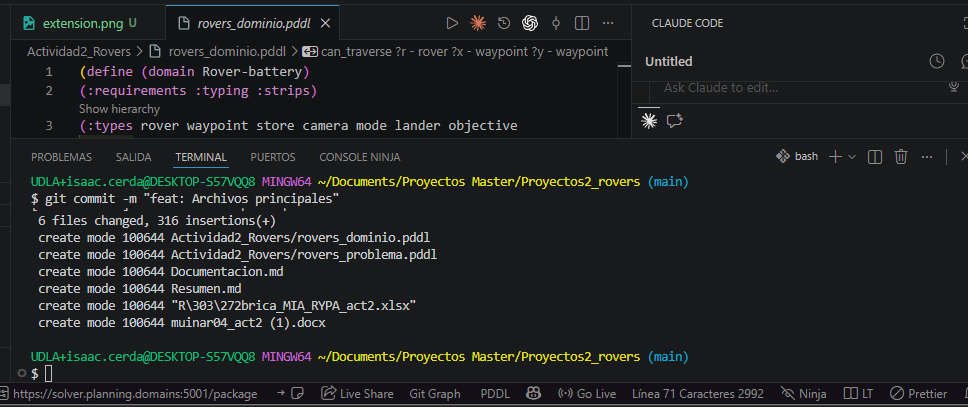
\includegraphics[width=0.85\textwidth]{act2_01_entorno_vscode.png}
\caption{Entorno de desarrollo: Visual Studio Code con los ficheros del
dominio y del problema abiertos.}
\label{fig:vscode}
\end{figure}

\begin{figure}[H]
\centering
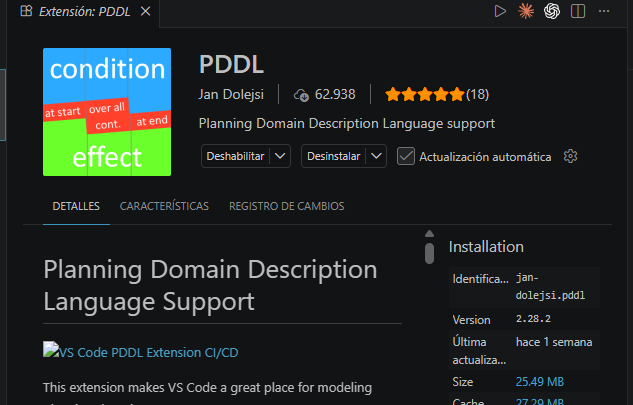
\includegraphics[width=0.85\textwidth]{act2_02_extension_pddl.png}
\caption{Extensi\'on PDDL de Jan Dolejsi (v2.28.2) instalada y activa.}
\label{fig:extension}
\end{figure}

\begin{figure}[H]
\centering
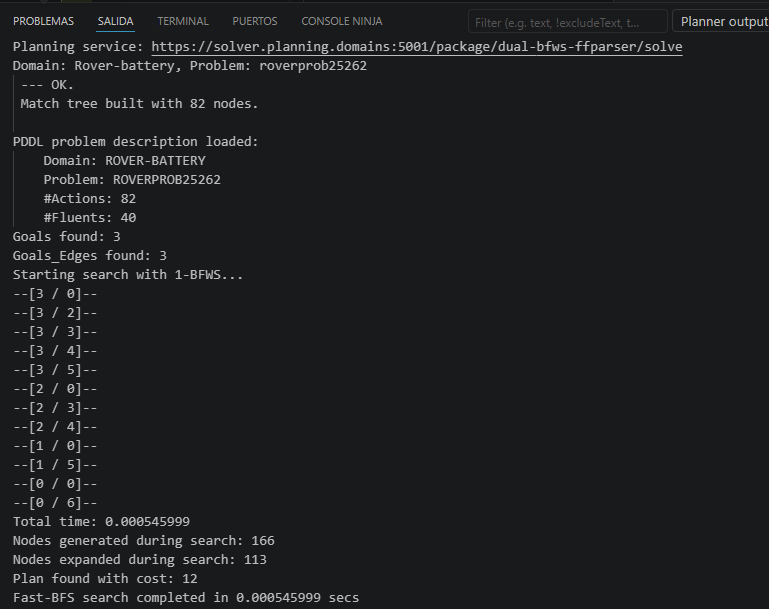
\includegraphics[width=0.85\textwidth]{act2_03_salida_planificador.png}
\caption{Traza del planificador sobre el caso base: nodos generados (166),
expandidos (113) y coste del plan (12).}
\label{fig:trazabase}
\end{figure}

\begin{figure}[H]
\centering
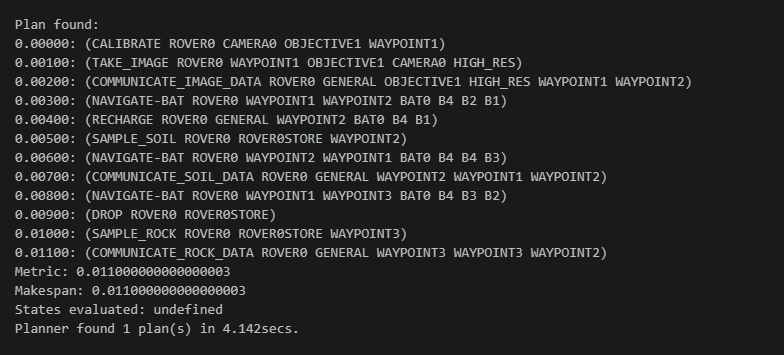
\includegraphics[width=0.85\textwidth]{act2_04_plan_encontrado.png}
\caption{Plan encontrado para el caso base (12 acciones).}
\label{fig:planbase}
\end{figure}

\begin{figure}[H]
\centering
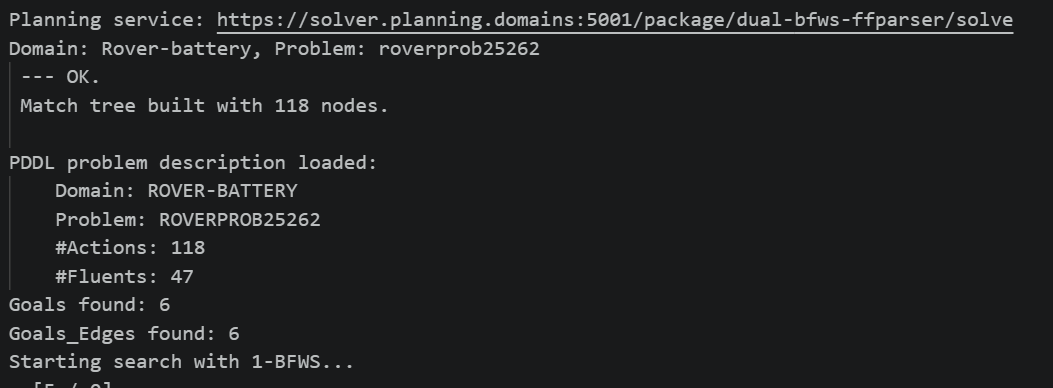
\includegraphics[width=0.95\textwidth]{act2_05_traza_21_plan.png}
\caption{Caso 2.1: plan generado por \texttt{dual-bfws-ffparser}
(coste 20).}
\label{fig:plan21}
\end{figure}

\begin{figure}[H]
\centering
\begin{subfigure}{0.48\textwidth}
  \centering
  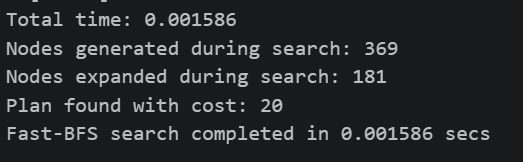
\includegraphics[width=\textwidth]{act2_06_traza_21_metricas.png}
  \caption{M\'etricas de b\'usqueda.}
\end{subfigure}\hfill
\begin{subfigure}{0.48\textwidth}
  \centering
  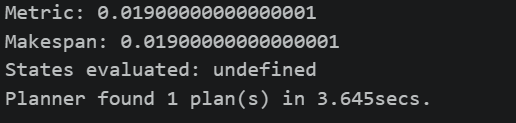
\includegraphics[width=\textwidth]{act2_07_traza_21_resumen.png}
  \caption{Resumen de la ejecuci\'on.}
\end{subfigure}
\caption{Caso 2.1: m\'etricas de la ejecuci\'on (369 nodos generados,
181 expandidos).}
\label{fig:metricas21}
\end{figure}

\begin{figure}[H]
\centering
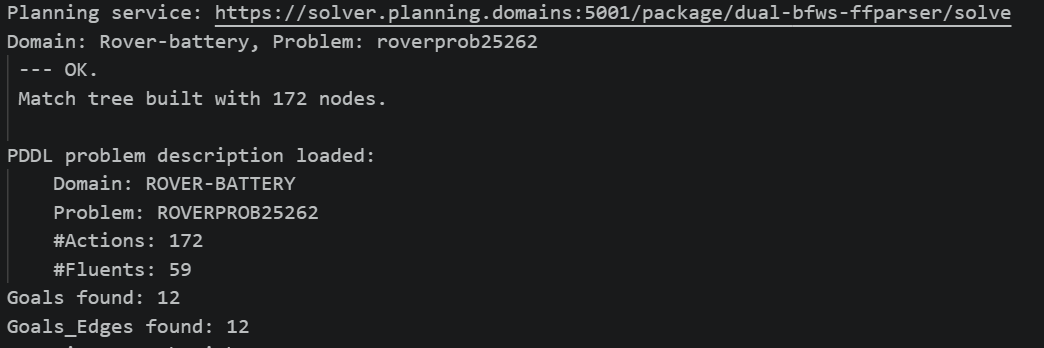
\includegraphics[width=0.95\textwidth]{act2_08_traza_22_plan.png}
\caption{Caso 2.2: plan generado por \texttt{dual-bfws-ffparser}
(coste 45).}
\label{fig:plan22}
\end{figure}

\begin{figure}[H]
\centering
\begin{subfigure}{0.48\textwidth}
  \centering
  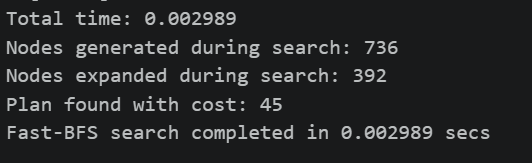
\includegraphics[width=\textwidth]{act2_09_traza_22_metricas.png}
  \caption{M\'etricas de b\'usqueda.}
\end{subfigure}\hfill
\begin{subfigure}{0.48\textwidth}
  \centering
  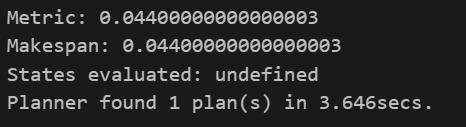
\includegraphics[width=\textwidth]{act2_10_traza_22_resumen.png}
  \caption{Resumen de la ejecuci\'on.}
\end{subfigure}
\caption{Caso 2.2: m\'etricas de la ejecuci\'on (736 nodos generados,
392 expandidos).}
\label{fig:metricas22}
\end{figure}

% TODO: anadir aqui la captura de la ejecucion de la Parte 4
% (rovers_parte4_dominio.pddl + rovers_parte4_problema.pddl),
% que actualmente es la unica evidencia visual que falta.
%
% \begin{figure}[H]
% \centering
% \includegraphics[width=0.95\textwidth]{act2_11_traza_parte4.png}
% \caption{Parte 4: ejecucion del nuevo dominio y problema. El plan de
% coste 10 comienza con la accion \texttt{tow\_lander}.}
% \label{fig:trazap4}
% \end{figure}

\end{document}
